\documentclass{report}
\usepackage{color}
\usepackage{amsmath,amssymb}
\usepackage[utf8]{inputenc}
\usepackage{graphicx}
\usepackage[english]{babel}
\selectlanguage{english}
\usepackage{hyperref}
\usepackage{booktabs}
\usepackage{mhchem}
%\usepackage{SIunits}
\usepackage{caption}
\renewcommand{\thetable}{\arabic{table}}

\usepackage{tabularx}
\usepackage{hyperref}
\usepackage{comment}
\usepackage{float}
\floatstyle{plaintop}
\restylefloat{table}
\DeclareMathSizes{10}{10}{9}{9}
\newcommand{\beq}{\begin{equation}}
% -- THIS COMMAND CREATES A SHORTHAND FOR \end{equation}
\newcommand{\eeq}{\end{equation}}
\newcommand{\of}[1]{\left(#1\right)}
\setlength{\textfloatsep}{5pt}
%\evensidemargin = 2pt
%\oddsidemargin = 2pt
\usepackage[top=1in, bottom=1.25in, left=0.85in, right=0.85in]{geometry}
%\usepackage{blindtext}
\usepackage{dblfloatfix}
\usepackage{tocloft}
\usepackage{afterpage}
\usepackage{dirtytalk}


\begin{document}


\begin{comment}

\title{\textbf{TFE4521 Specialization Project report 2017 Magnus Rammel}}
%\author{magnusrammel }
\nodate
\maketitle
\begin{Abstract}
\begin{center}
\textbf{Here is the abstract. }\\
\end{center}
\end{Abstract}


Fjern sectionnummer
Sidetall romertall først




\end{comment}

\pagenumbering{gobble}

%\topmargin = 5pt

\footskip = 0pt

%TFE4521 Specialization Project report 2017.

\title{\textbf{\Huge{HW/SW Codesign of a Pedestrian Detection System}} \newline \newline
by}
\author{\Large Magnus Rammel}


\begin{figure}[b]
    \begin{center}
        
\includegraphics[scale=0.32]{Attachments/NTNU.png}
        \caption{Department of Electronics and Telecommunications \\
        Norwegian University of Science and Technology}
        \label{AGCdiag}
    \end{center}
\end{figure}
\maketitle

\clearpage

\pagenumbering{roman}

\section*{Assignment text}
\addcontentsline{toc}{section}{\numberline{}Assignment text}

\textbf{Candidate name:} Magnus Rammel.\\\\
\textbf{Assignment title:} HW/SW Codesign of a Pedestrian Detection System. \\\\
\textbf{Assignment text:} \\
Advanced Driver Assistance Systems (ADAS) have become an integral part of modern high-end cars. With data from cameras and other sensors, they perform services such as pedestrian detection, blind spot detection, and lane departure warning. The computational requirements for many of the algorithms needed to process the data are substantial. To have price, size, compute and energy efficient solutions, a combination of hardware and software is typically required.  NTNU is partner in the EU research project Tulipp (Towards Ubiquitous Low-power Image Processing Platforms), where a system for pedestrian detection is one of the use-cases. A software implementation of the system is available in an open source repository. 
In this project assignment, the pedestrian detection system shall be investigated from a Hardware/Software Codesign perspective. Based on a literature study and early investigation of the system code, a design methodology shall be selected and described. Following the selected methodology, critical parts of the system shall be implemented in hardware using design tools suitable for Xilinx FPGAs. Overall improvement in performance and energy efficiency compared to an all software solution shall be estimated. To the extent time allows, test on an FPGA evaluation board shall be performed.\\\\
\textbf{Assignment proposer / Co-supervisor:} Snorre Aunet?, Norwegian University of Science and Technology.\\\\
\textbf{Supervisor:} Per Gunnar Kjeldsberg. \\\\\\\\\\


\noindent
\textit{\textbf{(Kommentarer markert med rødt skal fjernes, men inneholder beskrivelsene av underkapitlene fra itslearning og generelle kommentarer)}\\\color{red}\Big{Assignment text:}\\\\
\textbf{Candidate name:} your name here\\\\
\textbf{Assignment title:} the title goes here\\\\
\textbf{Assignment text:}\\
here you put the assignment text as given by your supervisor\\\\
\textbf{Assignment proposer / Co-supervisor:} here you put the name and contact information of the
person who has given the assignment (leave out if the assignment was given by you
department supervisor)\\\\
\textbf{Supervisor:} here you put the name of your supervisor from the department }\\
\clearpage

\section*{Abstract}
\addcontentsline{toc}{section}{\numberline{}Abstract}
Abstract
\\\\\\\\\\



\noindent
\textit{\color{red}\Big{Abstract:}\\
This is supposed to be a summary of the complete report. Include some sentences about the motivation for the work, background theory, and previous work. Then sum up in some more detail what your contribution has been and what you main results are. }\\
\clearpage


\afterpage{%/////begin afterpage/////
\newgeometry{top=0.5in, bottom=1.25in, left=0.85in, right=0.85in}




\section*{}
\addcontentsline{toc}{section}{\numberline{}Contents} %til listekomponenten

\renewcommand*\contentsname{Contents}%til overskrift på lista
\tableofcontents

\noindent
\textit{\color{red}\Big{Contents:}\\
This is the list of chapters and sub-chapter, including the page they start on. It is also often normal to include a list of figures, a list of tables, and a list with explanations of abbreviations, if you use a lot of them.}\\
\clearpage





\restoregeometry
}%/////end afterpage/////















\begin{comment}
% ... some material
\afterpage{%
\newgeometry{<options>}
% material for this page
\clearpage
\restoregeometry
} % end of \afterpage{...} material
% ... still more material
\end{comment}

\section*{Preface}
\addcontentsline{toc}{section}{\numberline{}Preface}
This specialization project has delivered a great learning outcome in terms of practical experience with previously acquired theoretical knowledge. The HW/SW Codesign topic was chosen partly due to its relevancy to my study programme specialization, but also because of the aforementioned practical learning outcome I assumed it would give me. The project has given me a deeper insight into the topic of HW/SW Codesign, as I expected it to.  \\
\noindent

\begin{comment}
Despite the learning outcome, the task accomplishment is less satisfactory than anticipated in terms of fulfillment of the project goals. The work process has often been slowed down due to specific tasks requiring more time to accomplish than anticipated, or due to encountering several unexpected problems in several areas related to the task that needed to be solved. Despite this, it is my belief that the accomplished results can be considered good enough in their own right.\\\\
\end{comment}

\noindent
I would like to thank my supervisor Per Gunnar Kjeldsberg for continually providing me with council on which steps to take forward project wise, as well as for giving feedback on the report at several instances during the project phase. \\\\\\\\


\noindent
\textit{\color{red}\Big{Preface:}\\
Here you can describe the process that led to the writing of this report (i.e., the project work process). Here you can mention why you chose this assignment and specific challenges you met with during your work. You can also thank people for help and support during this project.}\\
\\
\noindent
\subsection{Overview of report}
This report will describe a process that has been carried out to select an appropriate HW/SW Codesign methodology for certain applications of an existing Pedestrian Detection system. The report will start with an introductory part, which will be followed by a main  part in the middle, and finally a concluding part at the end. 
\\
\noindent
\subsubsection{Part 1: Introductory part}
The introductory part will contain the assignment text, as well as the abstract, preface and table of contents, in addition to this current chapter with introduction and motivation. The objective of the introductory part as a whole is to introduce the reader to the HW/SW Codesign philosophy, as well as to give a description of the project and the work process that has led to the finished report. 
\\
\noindent
\subsubsection{Part 2: Main part}
The main part begins with a chapter about the theory and background of HW/SW Codesign, which will describe the topic in theoretical detail. The part further continues with a chapter about some of the work that has been done on the topic in the past, before providing some information about the Pedestrian Detection system that is the basis for the work in this project. Following from this comes the measurements and results from the project work, which will contain graphs, tables and figures derived from the project work. 
Finally, the main part will feature a presentation of the chosen HW/SW Codesign methodology that is the result of the project work as a whole. 
\\
\noindent
\subsubsection{Part 3: Concluding part}
The concluding part will feature a chapter for discussions and one for conclusions, both in relation to the chosen methodology. It will thus debate whether or not the results are conclusive enough and if the methodology could have been improved in any way. 
\\
\noindent
\subsubsection{Part 4: Appendix}
At the bottom of the report there will be an appendix containing all graphs, figures, tables etc that were deemed too comprehensive or large in size to be included in the main parts of the report. 


\clearpage




\pagenumbering{arabic}

\chapter{Introductory part}
\section{Introduction and motivation}
%\addcontentsline{toc}{section}{\numberline{}Introduction and motivation}
Electronic gadgets of different shapes and sizes are a vital part of today's society. With ever increasing demands from the market for these gadgets, that require both increased performance as well as more advanced functionality, the need to increase the efficiency in the design process for these gadgets has become increasingly important for developers and producers. This efficiency increase is improtant to enable them to keep their position in the tough and highly competitive market. To accomodate the demands, several techniques for increasing the efficiency has been developed, and one particularly well regarded set of techniques is called Hardware/Software Co-design, or HW/SW Codesign for short. HW/SW Codesign is a design philosophy developed for the purpose of improving the cooperation between hardware and software of electronic applications, and utilizes the synergy between hardware and software to achieve this. 
\\\\
\noindent
The HW/SW Codesign philosophy is carried out by focusing on the concurrent design of hardware and software, in order to meet the given system-level objectives.\cite{ReadingsHWSW} 
With digital systems often being developed by several organizations and for different applications, the cooperation between the hardware and software parts within the system of these applications is not always considered optimal, which gives rise to a motivation for using the HW/SW Codesign philosophy. Notable HW/SW Codesign methods involve using digital HW design tools to design the hardware, as well as using simulation tools for testing the hardware in the design phase instead of the production phase. 
\\\\


\begin{comment}
This report will describe a process that has been carried out to select an appropriate HW/SW Codesign methodology for certain applications of an existing Pedestrian Detection system. The report will follow a traditional report structure. It starts with an introductory part, which will be followed by a main part in the middle, and finally a concluding part at the end. At the bottom of the report there will be an appendix containing all graphs, figures, tables etc that were deemed too comprehensive or large in size to be included in the main parts of the report. All measurements and results of the project will be described in the main part, while the concluding part will elaborate, discuss and conclude further on these topics, as well as propose recommendations for future work. 
\\\\\\\\
\end{comment}



\noindent
\textit{\color{red}\Big{Introductionandmotivation:}\\
This is normally Chapter 1 and gives an overview of the assignment and why this work is important. If you have chosen to focus mainly on a part of the assignment text, you may write something about this here and explain why. You also normally give a short description of the structure of the rest of the report towards the end of this chapter.  It is important to indicate which parts that are based on your own work. You may even include a list of your main contributions. }\\



\clearpage

\chapter{Main part}
\section{Theory and background}
%HWSW Codesign theory

HW/SW Codesign is, as mentioned in the introduction, a topic that has risen up in modern times in relation to the gradual development of electronic gadgets of different kinds. The book "A practical introduction to Hardware/Software Codesign" \cite{IntroHWSW} has the following definition of HW/SW Codesign: 
\\\\
\begin{center}
\say{
Hardware/Software Codesign is the design of cooperating hardware components and software components in a single design effort.
}
\end{center}
\hfill\break
\hfill\break
\noindent
%Til forord eller liknende: HWSW-teori vil i denne rapporten være svært grunnleggende og mindre omfattende, da rapportens formål er å presentere en løsning på et problem heller enn teori om temaet. 
This definition provides a short and accurate description of what the topic is about, and will be used as basis for defining the topic in this report. Based on this definition, one could also say that HW/SW Codesign is the process of deciding which tasks of a system that should be implemented in hardware and software. 
From a designers' point of view, implementing designs in software might be considered the easiest approach to follow. The reason for this is that software is often considered easy and flexible in terms of editing, and when complemented with access to fast compilers as well as software libraries and computers that are easy to come by, choosing software over hardware seems obvious. According to sources however, the choice of implementing in HW or SW is a lot more subtle in practice, as it tends to depend on several other factors in addition to the ease of access and editing. These factors are based on both technological reasons as well as economical ones, and will be outlined in more detail in the following subsections. 
\\
\noindent
\subsection{Performance factor}
One of the most vital technological factors to consider when making the decision between HW and SW for a system design is the performance one expects to receive from the implementation. One can for instance consider performance to be the amount of work done per unit time, where a unit of work is defined as the processing of 1 bit of data, and time is measured in clock cycles or seconds. Figure \ref{HWSWPerformance}, derived from \cite{IntroHWSW}, gives an illustration of the variations in performance for hardware and software, based on these considerations. 

\begin{figure}[H]
    \begin{center}
        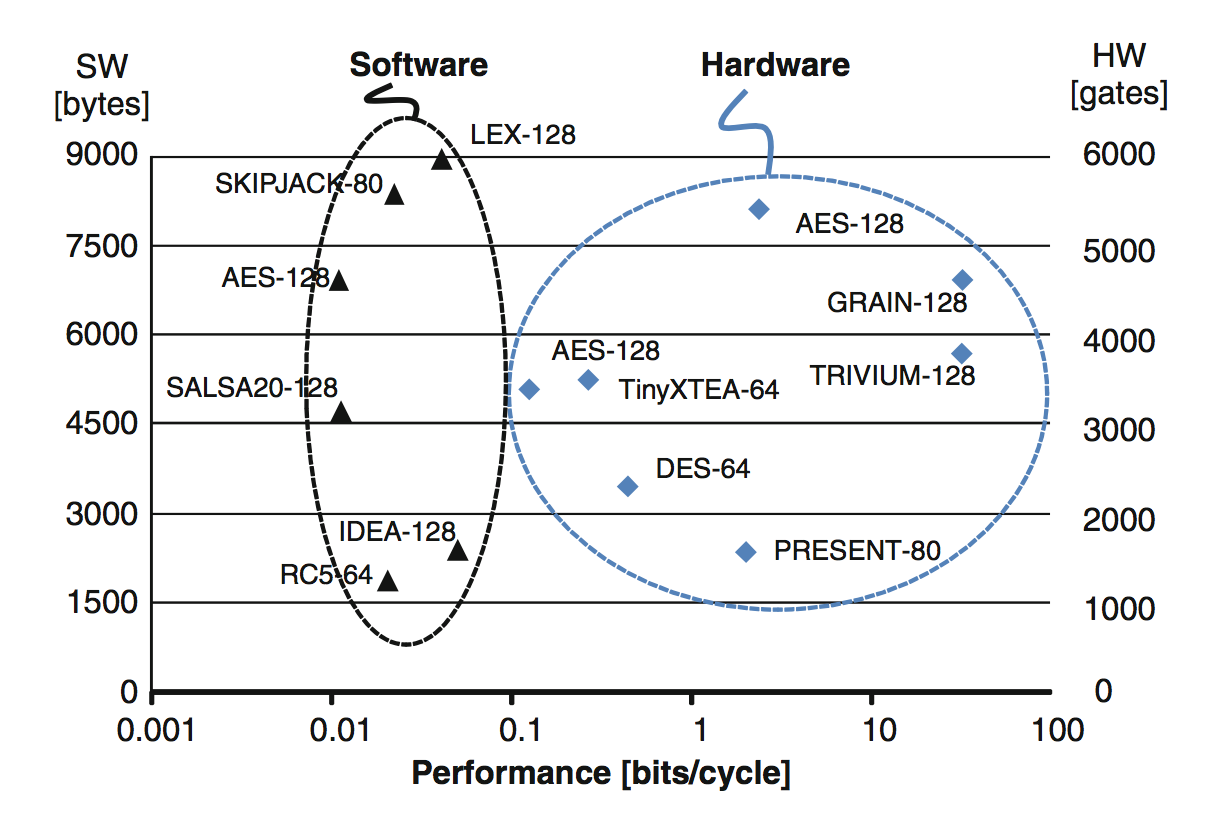
\includegraphics[scale=0.52]{Attachments/HWSWPerformance.png}
        \caption{Various cryptographic implementations in software and hardware proposed from the year 2003 to 2008 \cite{ReadingsHWSW}. }
        \label{HWSWPerformance}
    \end{center}
\end{figure}

\\\\
\noindent
The graph shows performance in bits per cycle. It demonstrates that, on average, hardware crypto-architectures
have a higher performance than embedded processors when one uses several different implementations for both HW and SW solutions. 
\\
Contrary to these results however, when one compares the clock frequency found in most hardware implementations to the clock frequency available in a processor executing a software implementation, the clock frequency in the processor may often outperform the one found in the hardware implementation. In this regard, the software implementation can achieve a higher performance than the hardware implementation simply because the processor performance outweighs the performance gained from the clock frequency and the parallel execution found in a corresponding hardware implementation. The decision between a hardware or software implementation based on performance therefore largely depends on the nature of the design task that is to be implemented, and in this sense whether the task is best suited to be executed in a parallel or a serial manner.  
\\
\noindent
\subsection{Energy efficiency}
Another technical factor to consider when choosing between hardware or software implementations is the aspect of energy efficiency or power consumption necessary for performing computations. Energy efficiency can be defined as the amount of useful work accomplished per unit of energy and is especially important to consider for portable battery operated applications. It is an established fact that increasing the energy efficiency results in a longer battery life, and this is intuitively a factor one seeks to have in portable battery operated applications. Figure \ref{Energyefficiency} gives an illustration of the amount of Gigabits possible to decrypt on each of the illustrated platforms, by using a single Joule of energy. 

\begin{figure}[H]
    \begin{center}
        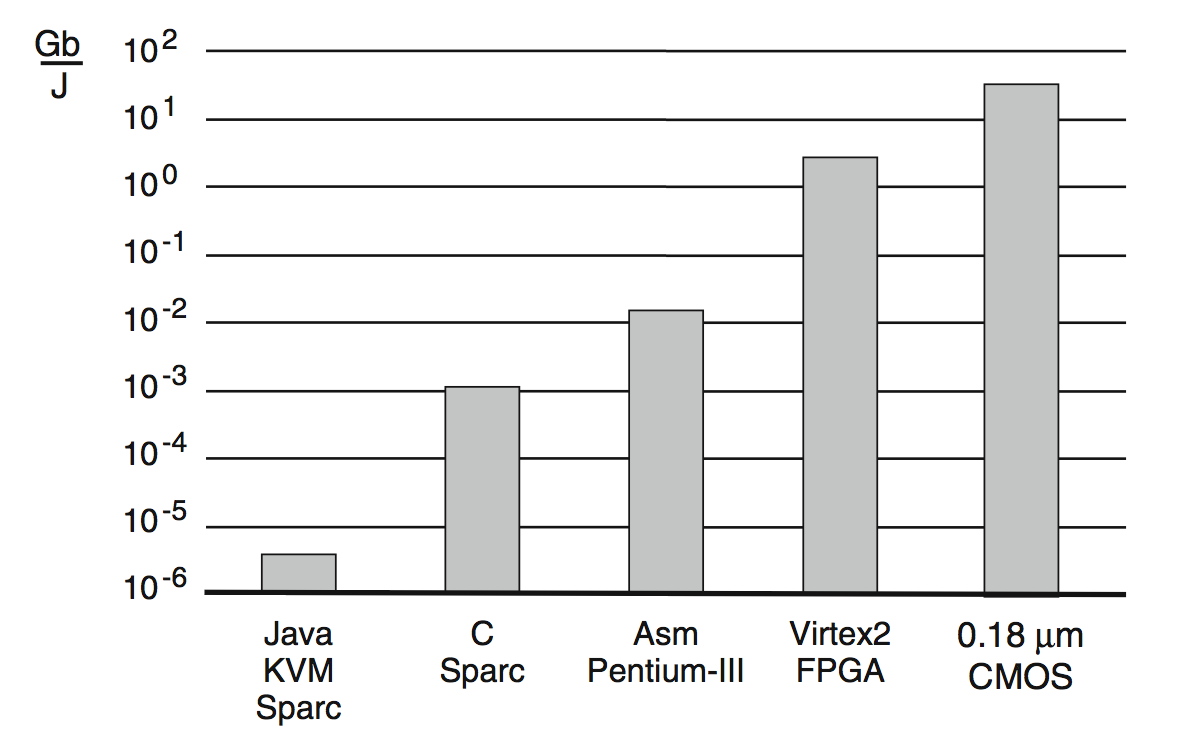
\includegraphics[scale=0.52]{Attachments/Energyefficiency.png}
        \caption{A particular encryption application used for different target platforms. }
        \label{Energyefficiency}
    \end{center}
\end{figure}

\noindent
The figure is meant to illustrate the amount of variation one can find in energy consumption for different target platforms. Despite the task being the same for all of the platforms, it can be seen from the figure that the amount of Gigabits decrypted for 1 Joule of energy varies over several orders of magnitude, which gives rise to a strong motivation for improving the energy efficiency as much as possible when designing a system. 
\\
\noindent
\subsection{Driving factors/Power density}
In the previous subsections it was outlined how a hardware implementation can usually outperform a software implementation and vice versa, and it was also pointed out how a system platform can have a power consumption that varies greatly in magnitude depending on the implementation used. This subsection will seek to give the full picture of what drives the hardware/software implementation decision by giving a short description of the other factors involved. 
\\
\noindent
As outlined previously, the performance and energy efficiency aspects of HW/SW Codesign generally favor a hardware design implementation over a software one because of the fixed and parallel nature of the former. Despite this fact, the design of modern electronic systems is characterized by the need to make a lot of trade-offs to achieve the optimal result for the given specification. Figure \ref{HWSWTradeoffs} displays a general overview of the trade-offs being made when choosing one over the other. 


\begin{figure}[H]
    \begin{center}
        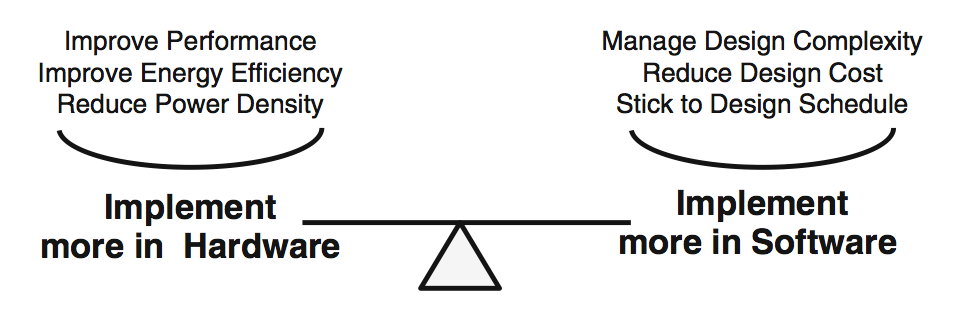
\includegraphics[scale=0.52]{Attachments/HWSWTradeoffs.png}
        \caption{The usual trade-offs needing to be made when choosing either a hardware- or a software implementation in the HW/SW Codesign philosophy. }
        \label{HWSWTradeoffs}
    \end{center}
\end{figure}
\hfill\break
\hfill\break
\noindent
Another factor involved in the implementation decision is therefore the power density or the power dissipation expected from a circuit. This factor is directly proportional to the clock frequency of a circuit, and thus applies to both hardware- and software implementations alike. In recent years the power density found in modern processors has reached a limit where modern cost-effective cooling technology can no longer keep up, and is unable to handle further increase in power. It is therefore believed that further performance increase cannot be achieved with increased clock frequency. The industry has therefore taken a large and fundamental shift towards parallel computer architectures. Examples of these architectures are Field Programmable Gate Arrays (FPGAs), Symmetric Multiprocessors (SMPs) and also dedicated processors for resource intensive tasks like graphics called Graphics Processing Units (GPUs).
\\
\noindent
\subsection{Design complexity}
The previous three subsections in this section have all presented factors for HW/SW implementations that favor hardware implementations. The factor of design complexity in modern systems however is one that is considered to be solved best with software, as flexible solutions that can easily be altered in the design without too much effort is favored over the fixed and hard coded nature of hardware implementations. This is evident when one looks at the complex attributes of modern electronic systems. To accommodate the design complexity in an optimal way, the aim is to make the implementation as flexible as possible, thus enabling the designer to alter the solution easily. The software is also used as a mechanism for creating higher levels of abstraction, to enable easier adjustments to future needs, and to solve problems with bugs. 
\\
\noindent
\subsection{Design cost}
Designing new chips is usually very expensive, which is why many hardware designers have begun making their chips programmable to enable them to be reused for different applications and multiple product generations. An example of this is the System on Chip (SoC) circuit, as well as FPGAs and others. 
\\
\noindent
\subsection{Shrinking design schedules}
It is usually always desirable to reduce the time needed to design a new electronic product. With new generations of electronic technology and applications continually bringing more complexity into the design, as well as replacing the older one quicker than before, the work load increases for the design engineer with each generation, which means that decreasing or shrinking the design schedules to complete the work in a shorter amount of time becomes necessary. In order to do this, the engineering teams attempt to work on multiple tasks at the same time, where hardware and software is then developed concurrently. As an example a software team will typically start development of the software to be run on the hardware as soon as the characteristics of the hardware is defined, and will begin before an actual prototype of the hardware is produced. 
\\
\noindent
\subsection{HW/SW Codesign space / Balancing}
With the previous subsections delving into the most prominent factors to consider for HW/SW Codesign, the art of making the optimal solution based on these factors is what the job of the design engineers is all about. The different trade-offs discussed also need to be put into the context of a design space. As can be derived from all the aforementioned factors, there are many different possible solutions for a design. The collection of all these solutions is called the HW/SW Codesign space, and is illustrated in a symbolic way in Figure \ref{HWSWDesignspace}. 


\begin{figure}[H]
    \begin{center}
        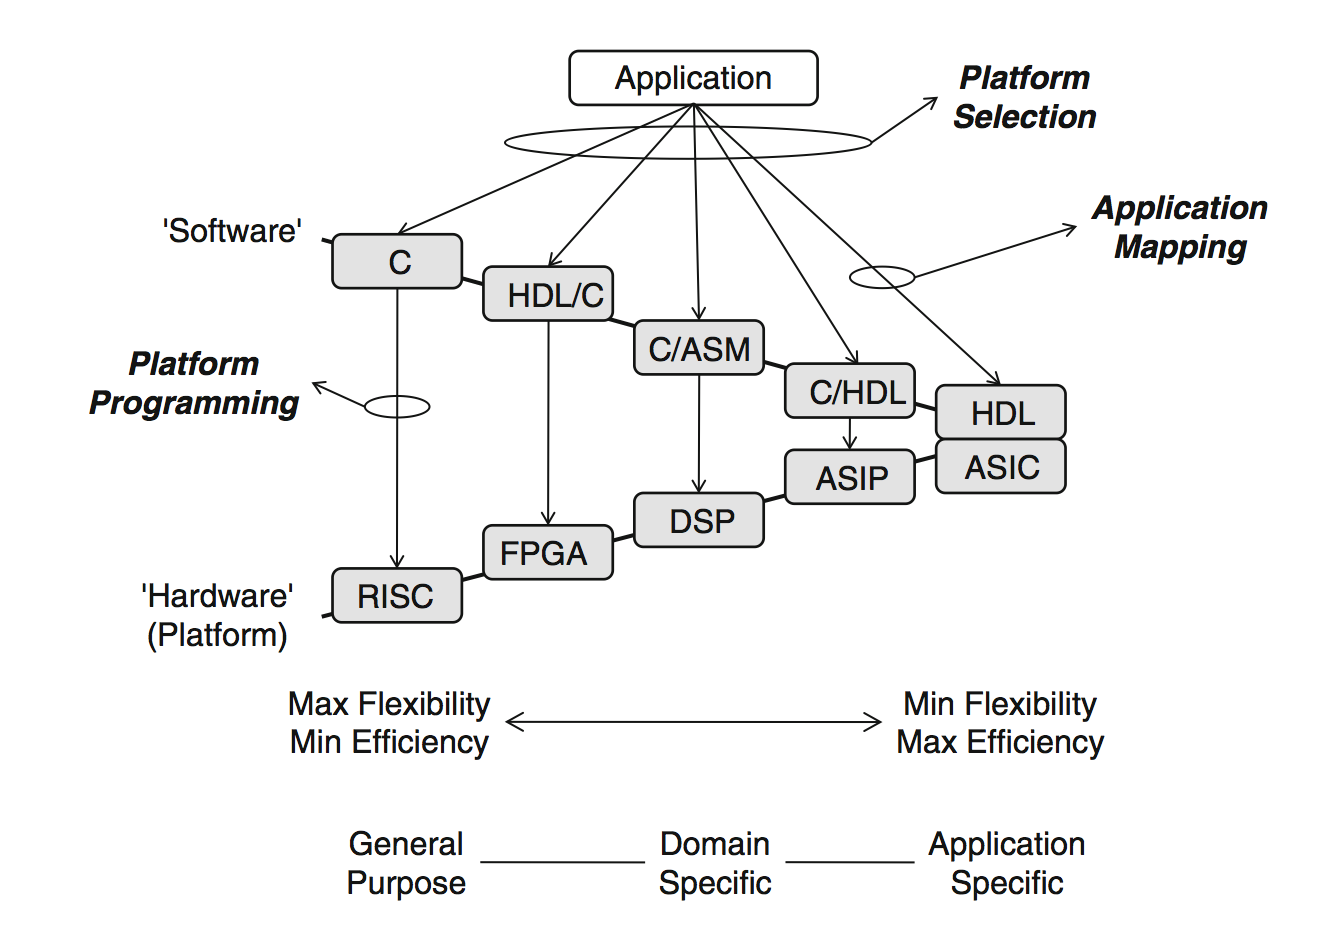
\includegraphics[scale=0.52]{Attachments/HWSWDesignspace.png}
        \caption{Illustration of the HW/SW Codesign space, outlined with the main activities. }
        \label{HWSWDesignspace}
    \end{center}
\end{figure}


\begin{comment}
In short terms, HW/SW Codesign seeks to increase the efficiency of electronic gadgets by improving the cooperation between the hardware and software of a system in the design phase. As mentioned in the introduction, this philosophy seeks to use the synergy normally found between hardware and software to improve the design of the system at an early stage. 
\\\\
\noindent
The book "A practical introduction to Hardware/Software Codesign" \cite{IntroHWSW} has the following definition for HW/SW Codesign: \\\\
\begin{center}
\say{
Hardware/Software Codesign is the design of cooperating hardware components
and software components in a single design effort.
}
\end{center}
\hfill\break
\hfill\break
\noindent
The nature of HW/SW Codesign can be considered as the process of finding the balance in the design for when to use hardware and when to use software to accomplish the tasks of a system. 
\\\\
\noindent
There are several key methods for carrying out the HW/SW Codesign philosophy in practice. One is to perform cosimulation of the hardware and software. 
\end{comment}





\section{Previous work}
Hva andre har gjort på feltet, f.eks. eksempler på andre designmetodikker. 

\section{Pedestrian Detection system}
This specialization project has used an application for a pedestrian detection system developed as part of the Tulipp project cite, and is used as basis for all the work and results outlined in this report. Since no further work to change the application was completed in this specialization project, the whole application in its entirety is the result of previous work performed by other project participants. The system used for the basis of this project's results consists of an online code repository that is meant to be compiled and run in the Linux computer operating system. Further details about the system are mentioned in the subsections below. 
\\\\

\subsection{Linux implementation}
%\addcontentsline{toc}{subsection}{\numberline{}6.1 - Linux implementation}
Something about how the project files are organized. Make files, Cmake, etc. \\\\

\subsection{System code}
%\addcontentsline{toc}{subsection}{\numberline{}6.2 - System code}
Some details about the languages used and basic notes on how they work. 
\\\\
\noindent
The previous code work completed for this application contains a great number of code files written in different languages, that are all used to make different test applications of the system run. %The test applications used as basis for this report is 
\\\\\\
\noindent
\textit{\color{red}\Big{Previous work:}\\
A description of what has been done before in this field. Also include background theory which is important to understand the work that is described later. Divide this into several chapters as needed. }\\
\clearpage




























\begin{comment}
\section{Previous work}
%\addcontentsline{toc}{section}{\numberline{}6 - Previous work}
This specialization project has used an application for a pedestrian detection system developed as part of the Tulipp project cite, and is used as basis for all the work and results outlined in this report. Since no further work to change the application was completed in this specialization project, the whole application in its entirety is the result of previous work performed by other project participants. The system used for the basis of this project's results consists of an online code repository that is meant to be compiled and run in the Linux computer operating system. Further details about the system is mentioned in the subsections below. 
\\\\

\noindent
\textit{\color{red}\Big{Previous work:}\\
A description of what has been done before in this field. Also include background theory which is important to understand the work that is described later. Divide this into several chapters as needed. }\\

\subsection*{6.1 - Linux implementation}
\addcontentsline{toc}{subsection}{\numberline{}6.1 - Linux implementation}
Something about how the project files are organized. Make files, Cmake, etc. \\\\

\subsection*{6.2 - System code}
\addcontentsline{toc}{subsection}{\numberline{}6.2 - System code}
Some details about the languages used and basic notes on how they work. 
\\\\
\noindent
The previous code work completed for this application contains a great number of code files written in different languages, that are all used to make different test applications of the system run. %The test applications used as basis for this report is 

\clearpage
\end{comment}



\section{Project work}
%\addcontentsline{toc}{section}{\numberline{}7 - Project work}
This section will describe all the work accomplished by the student in this specialization project. The project has lasted for 93 week days and has been continually worked on from the start, albeit in parallel with other courses as usual for this kind of project. 
\\\\

\noindent
\textit{\color{red}\Big{Your work:}\\
N chapters describing your own work. It can be natural to use a tree structure, where the first chapter gives an overall introduction and the remaining chapters with sub-chapters describes details. In some cases it is natural to partition procedure and results in different chapters, in other cases this is not natural.}\\


\subsection{Measurements/Measurement tools}
%\addcontentsline{toc}{subsection}{\numberline{}7.1 - Measurement/Measurement tools}
Valgrind tools, other tools, principles, etc. Maybe add more subsections because of this. \\

\subsubsection{Callgrind}
%\addcontentsline{toc}{subsubsection}{\numberline{}7.1.1 - Callgrind}
Basic information, what it can be used for. \\

\subsubsection{Massif}
%\addcontentsline{toc}{subsubsection}{\numberline{}7.1.2 - Massif}
Basic information, what it can be used for. \\

\subsubsection{etc}
%\addcontentsline{toc}{subsubsection}{\numberline{}7.1.3 - etc}
etc\\\\\\

\subsection{Results}
%\addcontentsline{toc}{subsection}{\numberline{}7.2 - Results}
Measurement results. \\

\subsubsection{Callgrind results}
%\addcontentsline{toc}{subsubsection}{\numberline{}7.2.1 - Callgrind results}
Presented with graphs, tables (maybe in 11 - Appendix if too big), figures etc, and written in a more or less straight forward way. Elaboration saved for 8 - Discussion.\\

\subsubsection{Massif results}
%\addcontentsline{toc}{subsubsection}{\numberline{}7.2.2 - Massif results}
Presented with graphs, tables (maybe in 11 - Appendix if too big), figures etc, and written in a more or less straight forward way. Elaboration saved for 8 - Discussion.\\

\subsubsection{etc}
%\addcontentsline{toc}{subsubsection}{\numberline{}7.2.3 - etc}
etc\\\\\\

\subsubsection{Suggested HW/SW Co-design methodology}
%\addcontentsline{toc}{subsection}{\numberline{}7.3 - Suggested HW/SW Co-design methodology}
Description of methodology in detail, probably with more subsections. Maybe even include
\\


\clearpage

\chapter{Concluding part}
\section{Discussions}
%\addcontentsline{toc}{section}{\numberline{}8 - Discussions}
Some points about the choice of methodology perhaps\\
Getting system to run in linux, took more time than estimated \textit{\color{red} - Fjerne?}\\
Simulation in Xilinx Vivado, why did not accomplish \textit{\color{red}- Flytte til Conclusion?}\\
Implementation on FPGA, why did not accomplish \textit{\color{red}- Flytte til Conclusion?}\\\\
\cite{PacketBased, Packets}
\\\\
\noindent
\textit{\color{red}\Big{Discussions:}\\
Here you should discuss the results you have achieved. What did not end up the way you wanted and why? What would you have done differently if you started from scratch again? }\\


\subsection{Compilation struggles}
%\addcontentsline{toc}{subsection}{\numberline{}8.1 - Compilation struggles}
Issues\\


\subsection{Measurement issues/problems, if any}
%\addcontentsline{toc}{subsection}{\numberline{}8.2 - Measurement issues/problems, if any}
Issues/dissatisfactions with Callgrind, Massif, etc. \\

\clearpage



\section{Conclusions}
%\addcontentsline{toc}{section}{\numberline{}9 - Conclusions}
Conclusions
\\\\\\\\
\noindent
\textit{\color{red}\Big{Conclusions:}\\
Not like the abstract, the conclusions should focus (more or less) solely on the results you have achieved. Sometimes it is natural to combine this with the discussion.  Here it is also normally a good idea to include indications of future work.}\\
\clearpage



\section{Bibliography}
%\addcontentsline{toc}{section}{\numberline{}10 - Bibliography}
\bibliographystyle{unsrtnat}
\bibliography{Bibliography.bib}
\\\\\\\\
\noindent
\textit{\color{red}\Big{Bibliography:}\\
This can alternatively be placed at the very end, after the appendixes. There are a number of "schools" for the bibliography. In a report it is normally best to make the list alphabetically according to the name of the first author. For references you may either use numbers [1] or a letter combination of author names and year [NLK02].
Appendix. This is where you put everything that is not needed to read in detail to understand the rest of the report, but which should still be included for completeness. Examples are source code, data sheets, detailed synthesis results etc.}\\
\clearpage

\section{Appendix}
%\addcontentsline{toc}{section}{\numberline{}11 - Appendix}
Tables, graphs, figures etc from the measurement results that are considered too big to include in report sections. 




\end{document}
